
BOUT++ \cite{BOUT++,boutwebsite} is a framework for writing fluid and plasma simulations in curvilinear
geometry. 
It is designed primarily to target reduced plasma fluid models, but it can
evolve any number of partial differential equations, with equations appearing
in a readable form via its domain specific language.
BOUT++ is being used in Project \nep\ as the framework in which to build the
fluid referent model proxyapp.

A team of BOUT++ developers 
%(Joseph Parker, Peter Hill, David Dickinson and Benjamin Dudson) 
attended the three VECMAtk hackathons in Spring 2021.
The goal of the hackathon work was to create the software framework to enable
BOUT++ to use VECMAtk,
and to develop workflows for uncertainty quantification and the creation of
surrogate models.
In this report we focus on the development of the software infrastructure and
the workflows for uncertainty quantification.
The code produced at the hackathons is available in the repository \cite{bout_vecma_repo}.

\subsection{Software Infrastructure}\label{sec:VECMA}

The VECMA toolkit wraps around user's software, providing a library of python
functions for non-intrusive UQ.
From VECMAtk's perspective, BOUT++ is a black box code to which it must
provide input parameters and from which it must read output quantities of
interest (QoIs).
Therefore the workflow is written in Python,
and is driven by calls to VECMAtk functions.
VECMAtk selects the parameter values to be sampled,
collects the QoI values, 
and calculates and plots statistical quantities such as Sobol indices and
confidence intervals.
The only necessary interaction between VECMA and BOUT++ is for VECMA to
communicate input parameters to BOUT++ and to read back output values.
This is achieved by providing an \emph{encoder}, a routine that is capable of
writing BOUT++ input files,
and a \emph{decoder}, a routine to parse BOUT++ output files.
Both are actually classes providing additional functions, such as routines to
check that BOUT++ simulations have finished.
Examples of decoders and encoders used for BOUT++ are given in Appendices \ref{sec:bout_decoder} and \ref{sec:bout_encoder} respectively.

This framework structure makes it very easy to reuse the same workflow with
different codes.
BOUT++ could be replaced by any other code that produces the same QoIs from the
same parameters simply by replacing the BOUT++ encoder/decoder with
corresponding functions for that other code.

This pattern also makes it easy to use synthetic data instead of an actual
code execution.
Instead of calling the encoder/decoder, one simply calls a function to return
the QoIs as a function of parameters.
This is particularly useful in developing the workflow, such as testing the
sampling routines or plotting functions, as executing BOUT++ is by far the
most significant runtime cost in the workflow. 

The encoders/decoders also provide the method for changing the QoIs for
different physical cases.
For example in our work with temperature $T(x,y,z,t)$ as the QoI,
each of the different cases -- fixed point over time $T(0,0,0,t)$,
spatial range at the final time $T(x,0,0,t_{\mathrm{end}})$,
or logarithm of temperature $\log[T(x,0,0,t_{\mathrm{end}})]$ --
were each achieved by implementing a separate decoder.\footnote{A similar
approach allowed us to work around a bug in the \texttt{chaospy} sampling routine
(a library dependence of VECMAtk).
The chaospy log-uniform probability distribution was broken, but the uniform
distribution was functional.
Therefore, in order to obtain a log-uniform distribution, we provided an encoder that wrote input parameter \texttt{p}
to the BOUT++ input file as \texttt{variable=10**p} instead of \texttt{variable=p}.}

\subsection{Uncertainty Quantification}\label{sec:uqsurrogate}

The first workflow considered introduced UQ into BOUT++ simulations.
Instead of performing a single simulation to obtain a single result, the
VECMAtk UQ framework performs an ensemble of simulations, varying chosen
input parameters in a specified range.
From this, VECMAtk fits a surrogate model: it finds the QoIs as a function of
the input parameters.
With this model it calculates statistics, such as the mean value of a QoI and
corresponding confidence intervals, and the Sobol indices, which give a way
of quantifying how much uncertainty in the QoIs is due the variation of each
parameter.

One-dimensional heat conduction was used as an initial test problem,
\begin{align}
\frac{\partial T}{\partial t} = \chi \frac{\partial^2T}{\partial x^2},
\label{eq:heat_conduction}
\end{align}
where $T$ is the temperature on the spatial domain $x\in[0,1]$
with boundary conditions $T(0,t)=T(1,t)=0$ and initial condition 
$T(x,0) = T_0\exp[-(x-0.5)^2/0.04]$.
Here, the thermal conductivity $\chi$ and the initial amplitude $T_0$ are uncertain parameters. 

\subsubsection{Polynomial chaos expansion}\label{sec:PCE}

\begin{figure}[tbp]
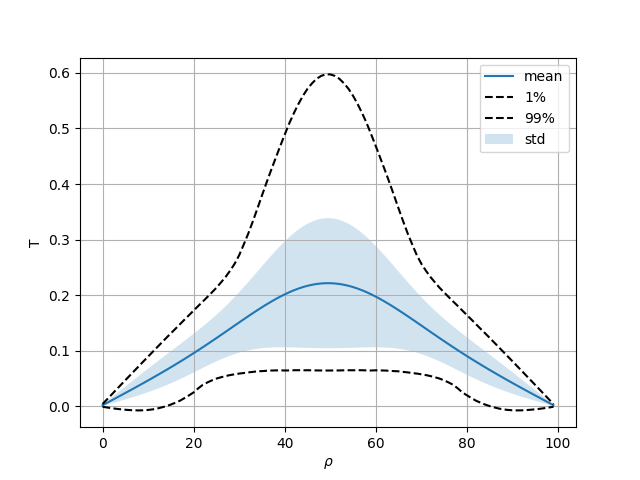
\includegraphics[width=0.5\textwidth]{T_vs_x_mean_ci.png}
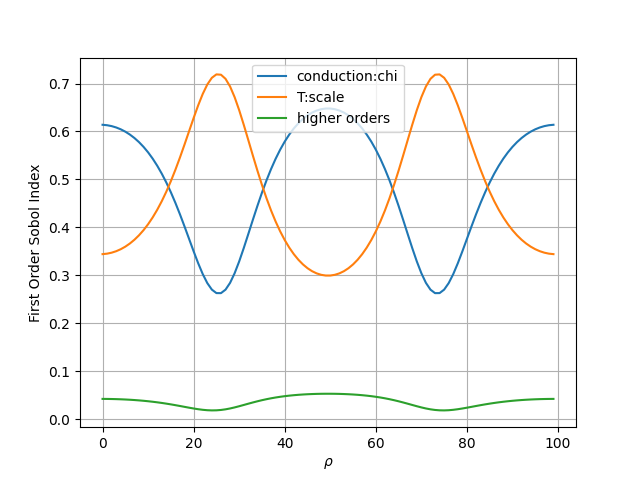
\includegraphics[width=0.5\textwidth]{T_vs_x_sobols.png}
%%%\includegraphics[width=0.5\textwidth]{log_T_vs_x_mean_ci.png}
%%%\includegraphics[width=0.5\textwidth]{log_T_vs_x_sobols.png}
\caption{%
Mean and confidence intervals (left) and Sobol indices (right) plotted
against $x$ array index for quantity of interest $T$. 
%%%Mean and confidence intervals (left) and Sobol indices (right) plotted
%%%against $x$ array index for quantity of interest $T$ (top) and $\log(T)$
%%%(bottom). 
\label{fig:conduction}
}
\end{figure}

As a first example, we implemented a workflow for 1D heat conduction
\eqref{eq:heat_conduction} varying $\chi\in(0.2,4)$ and $T_0\in(0.5,1.5)$
using polynomial chaos sampling.
The resulting statistics and Sobol indices for $T$ at the final time $T=10$ is shown in %the top row of 
Figure\ \ref{fig:conduction}.
The left figure shows the mean final temperature and its confidence intervals
.
The right figure shows the first Sobol indices, which describe how much of the
uncertainty is due to each parameter.
For example, at the centre of the domain, about $65\%$ of the uncertainty is
due to varying $\chi$ (independently of $T_0$), about $30\%$ is due to varying
$T_0$ (independently of $\chi$), and the remaining $5\%$ is due to varying both
in a coupled fashion.

The statistics are qualitatively converged using only a 3rd-order polynomial
chaos expansion which requires $(3+1)^2=16$ code evaluations in two
dimensions.
However the confidence intervals encompass negative values of temperature
near the boundary, even though the temperature is non-negative and all
simulation data provided is also non-negative.

One approach fixing this is to use $\log(T)$ as the QoI.
The logarithm is a bijective map between the positive-valued temperature
$T\in(0,\infty)$ and the real value $\log(T)\in(-\infty,\infty)$.
Therefore this allows the same analysis routines to be performed on $\log(T)$
without concern about sign.
The resulting confidence intervals now only allow positive temperatures.
Moreover the Sobol indices are qualitatively the same,
indicating that the transformed model ascribes uncertainty to the various
parameters in a similar fashion.

However, considering higher-order polynomial chaos it becomes apparent that
the negative values are an artefact of the data analysis routine.
Near $T=0$, the temperature is a steeply-varying function of the input
parameters, and low-order polynomial fitting is simply inaccurate, predicting
negative values.
Increasing the order of the polynomial fit (by increasing the order of PCE
and providing more simulation data) leads to this problem's no longer being
observed.

\subsubsection{Adaptive stochastic collocation}\label{sec:asc}

Using higher-order polynomial chaos is reasonable when varying a small number
of parameters, but varying more parameters is beset by the ``curse of
dimensionality'': the number of samples needed for $n$th-order PC with $d$ parameters is $(n+1)^d$.
Therefore, we also implemented EasyVVUQ's sampling with adaptive stochastic
collocation (ASC), which is based on the algorithm by Gerstner and Griebel
\cite{Gerstner03}

In ASC, the grid of sampling points for each parameter is adaptively refined,
beginning from a grid with only one sampling point for each parameter.
Estimates are made for the reduction in the error that would result from
adding one more sampling point in each parameter;
the refinement is made to the parameter which would reduce the error the most.
As a result, computing resources are directed where they are most effective,
yielding results that are comparable with high-order PCE but which require
many fewer code evaluations.

Implementing a new sampling algorithm (from a VECMA user's perspective) is a
simple matter of changing the class on which sampling routines are called.
However, adaptive stochastic collocation allows additional functionality which
we may incorporate in our workflow.
In particular, ASC uses a Clenshaw--Curtis collocation grid which has a nested
quadrature grid (unlike in Gaussian quadrature, the grid for $(n+1)$th order
accuracy contains all the points for $n$th order accuracy).
This means we may increase the order of accuracy by adding one new code
evaluation, rather than $(n+1)$ as would be required in PC.
This allows us to use an iterative approach, continuing to refine the order in
each parameters dimension until some convergence criteria is met.
In our workflow, we used relative changes in the Sobol indices from one
iteration to the next, but this criterion is not ideal as it is noisy and
non-monotonic.

\newcommand{\pd}[2]{\frac{\partial #1}{\partial #2}}
\newcommand{\tpd}[2]{\partial #1/\partial #2}
\newcommand{\tpdd}[2]{\partial^2 #1/\partial #2^2}
Finally, as a proof of concept we implemented uncertainty quantification for
a two-dimensional simulation of plasma filament propagation, 
\begin{subequations}
\label{eq:blob2d}
\begin{align}
	\pd{n}{t} &= -\{\phi, n\} + 2\frac{\rho_s}{R_c} \pd{n}{z} % // Curvature term
	              + D_n \nabla^2n,  \label{eq:density} \\ %;                // Diffusion term
\pd{\Omega}{t} &= -\{\phi, \Omega\} + 2\frac{\rho_s}{R_c} \pd{n}{z} % * (rho_s / R_c) / n     // Curvature term
		+ \frac{D_{\Omega}}{n} \nabla^2 \Omega,  \label{eq:omega} \\%         // Viscous diffusion term
\nabla^2 \phi &= \Omega, \label{eq:vorticity}
\end{align}
\end{subequations}
in a two-dimensional box $(x,z)$ with Dirichlet boundary conditions in $x$ and periodic boundary conditions in $z$.
In \eqref{eq:blob2d}, $n$ is plasma density, $\Omega$ is vorticity, $\phi$ is
electrostatic potential, $t$ is time,
$\rho_s$ is the Bohm gyroradius,
$R_c$ is the radius of curvatuve,
$D_n$ and $D_{\Omega}$ are dissipation parameters,
and
$\{A,B\} = (\tpd{A}{x})(\tpd{B}{z}) - (\tpd{A}{z})(\tpd{B}{x})$ is a Poisson bracket.
We use the two-dimensional Laplacian $\nabla^2 \equiv \tpdd{}{x}+\tpdd{}{z}$.
Between each timestep, the vorticity equation \eqref{eq:vorticity} must be solved for $\phi$ so its value can be used in \eqref{eq:density} and \eqref{eq:omega} to advance $n$ and $\Omega$.
We use $\phi$ at the current timestep as an initial guess for the iterative method (and $\phi=0$ as the guess for the first time step).

Four input parameters were varied, the constant coefficients $\rho_s$, $R_c$,
$D_n$ and $D_{\Omega}$.
While still reasonably small, individual simulations require around 10 minutes
on 16 cores on the University of York's cluster.
Third order PCE required 1296 simulations, while comparable results using ASC
only required 256 simulations.

%%%\begin{figure}[tbp]
%%%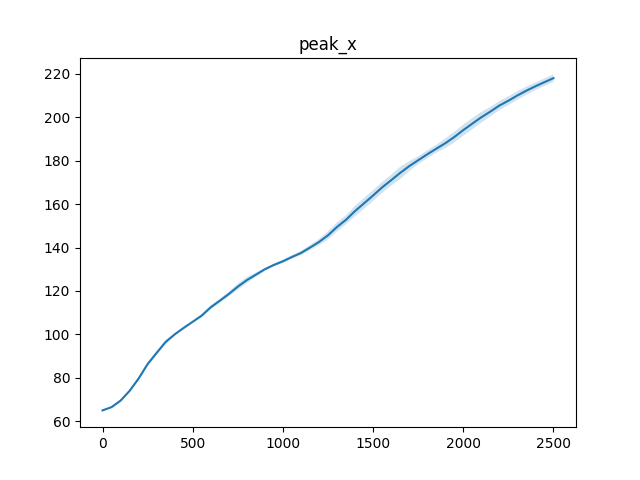
\includegraphics[width=0.5\textwidth]{peak_x_moment.png}
%%%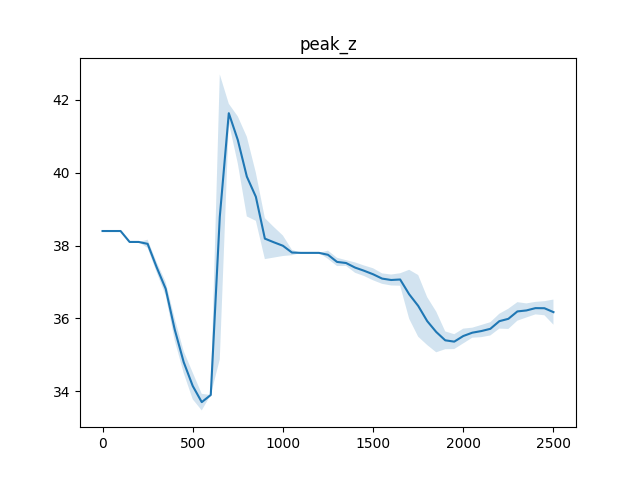
\includegraphics[width=0.5\textwidth]{peak_z_moment.png}
%%%%%%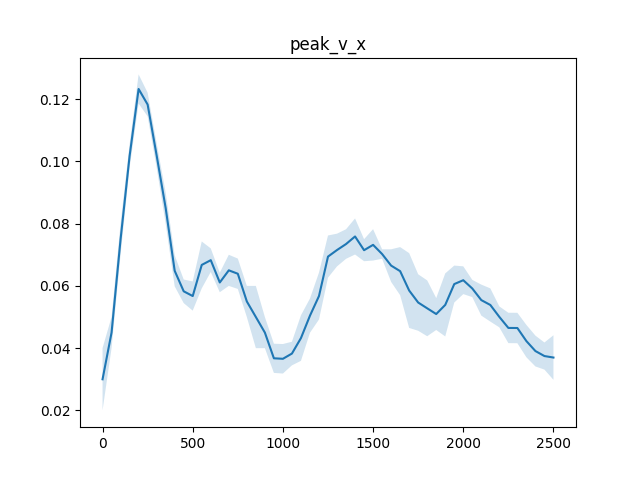
\includegraphics[width=0.5\textwidth]{peak_v_x_moment.png}
%%%%%%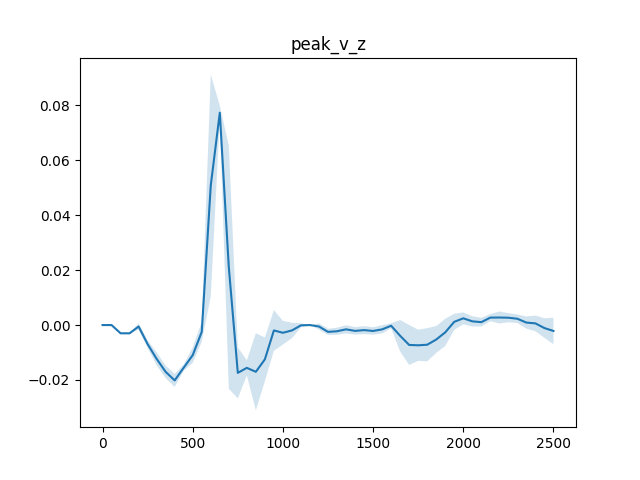
\includegraphics[width=0.5\textwidth]{peak_v_z_moment.png}
%%%\caption{%
%%%	The grid cell containing the peak of a plasma filament in $x$ (left) and $z$
%%%	(right) against timestep.
%%%The line shows the mean and shaded region shows the [10\%,90\%] confidence intervals.
%%%%%%Mean and confidence intervals (left) and Sobol indices (right) plotted
%%%%%%against $x$ array index for quantity of interest $T$ (top) and $\log(T)$
%%%%%%(bottom). 
%%%\label{fig:filament}
%%%}
%%%\end{figure}

% Notes on developing surrogate models
% Omitted for length
%%%\subsection{Surrogate models}
%%%
%%%Turning to surrogate models.
%%%Useful for developing, e.g. subgrid turbulence model.
%%%Specific case develop surrogate model for performance data.
%%%In BOUT++, often need iterative solvers for time advance and Poisson solver whose parameters (e.g. convergence tolerances) can interact in non-trivial fashion.
%%%As base case, considered varying two parameters, $a$ the absolute tolerance and $r$ the relative tolerances for the convergence of the time advance,
%%%and measuring the resulting error and run time in the simulation.
%%%Ideally, one would use a small number of simulations to build a surrogate
%%%model for error and run time as as function of input parameters, to inform parameter selection.
%%%
%%%In this case, the parameters are known to influence the error at the end of the simulation as follows,
%%%\begin{align}
%%%\label{eq:error}
%%%E \sim 
%%%\begin{cases}
%%%r^{0.75}, \hspace{1cm} a < T_0 r\\
%%%a^{0.75}, \hspace{1cm} a > T_0 r
%%%\end{cases}
%%%\end{align}
%%%where $T_0$ is some constant that characterizes the magnitude of the solution
%%%$T$.
%%%This function has a number of features that makes it interesting as a test for surrogate models.
%%%Firstly, the function contains a phase transition from constant to
%%%non-polynomial law behaviour (as one varies one parameter with the other
%%%fixed).
%%%Secondly, the parameters can reasonably take any in the range $a,r\in[1e-14,1]$ so are best treated by varying them on a logarithmic scale.
%%%The error is also best characterised on a logarithmic scale.
%%%Finally, the error from the code is very noisy -- there are significant random fluctuations on top of the function \eqref{eq:error}.
%%%
%%%\subsubsection{Polynomial chaos expansion}
%%%
%%%1D scan - fix $r=10^{-6}$, scan in $a$.
%%%
%%%Really important to use log-log scale.
%%%
%%%Doing so, get qualitatively good fit at low order.
%%%However, as PCE interpolates the data, the model overfits and becomes extremely oscillatory at high order.
%%%This means one does not actually improve the quality of the surrogate model by including more data.
%%%
%%%PCE also requires many samples, which will become prohibitively expensive as we increase the number of input parameters.
%%%
%%%\subsubsection{Adaptive stochastic collocation}
%%%
%%%Adaptive stochastic collocation sampling reduces the number of data samples needed but still overfits the data.
%%%
%%%\subsubsection{Artificial neural networks}
%%%Implemented ANN for the model using EasySurrogate.
%%%
%%%Improved model for data as no longer interpolates data, but requires $\sim
%%%50\%$ of data points to be accurate.
%%%
%%%\subsubsection{Gaussian processes}
%%%
%%%Gaussian processes using EasyVVUQ's interface to the \texttt{sklearn} library produced the best results.
%%%
%%%%Const * Matern($\nu=1.5$) + WhiteNoise
%%%
%%%Good fit with $\sim 5\%$ of the data used.
%%%
%%%However requires sensible kernel choice, is sensitive to initial guess of hyperparameters (and can fail without good guesses), and sensitive to sampling points.
%%%
%%%
%%%
%%%
%%%
%%%
%%%	
%%%
%%%
%%%
